
%% bare_jrnl.tex
%% V1.4
%% 2012/12/27
%% by Michael Shell
%% see http://www.michaelshell.org/
%% for current contact information.
%%
%% This is a skeleton file demonstrating the use of IEEEtran.cls
%% (requires IEEEtran.cls version 1.8 or later) with an IEEE journal paper.
%%
%% Support sites:
%% http://www.michaelshell.org/tex/ieeetran/
%% http://www.ctan.org/tex-archive/macros/latex/contrib/IEEEtran/
%% and
%% http://www.ieee.org/

\documentclass[12pt,a4paper,journal]{IEEEtran}

\usepackage{graphicx}
\usepackage{xcolor}
\usepackage{listings}

\lstset{
        keywordstyle=\color{blue}, 
        commentstyle=\color[cmyk]{1,0,1,0}, 
        frame=single, 
        escapeinside=``, 
        breaklines=true, 
        basicstyle=\small\ttfamily,
        extendedchars=false, 
        xleftmargin=2em,xrightmargin=2em, aboveskip=1em, 
        tabsize=4, 
        showspaces=false 
       }

\begin{document}

\title{Chromatic Pad Controlled by Music}


\author{Qiming~Guo,
        Chuhan~Min,
        and~Shuyao~Xie% <-this % stops a space
        }


% The paper headers
\markboth{University of Pittsburgh, ECE embedded computer system design final project}%
{Shell \MakeLowercase{\textit{et al.}}: Bare Demo of IEEEtran.cls for Journals}

% make the title area
\maketitle

% As a general rule, do not put math, special symbols or citations
% in the abstract or keywords.
\begin{abstract}
The project will be concerned in designing and building a colorful pad built by LEDs. The system will consist of a microprocessor that will control the LED display, a Spectrum Shield that will split an audio signal into 7-bands which could be read by ADC and a LED Pad made by ourselves will show music visually. Software will be designed to implement the functions using C. 
\end{abstract}

% Note that keywords are not normally used for peerreview papers.
\begin{IEEEkeywords}
spectrum analyzing, LED driving
\end{IEEEkeywords}

\section{Introduction}
\IEEEPARstart{M}{usic} is one of the most essential components in our life. People play music by different situations, different spirit, different culture. Some people believe that they cannot live without music. Music could provide us with relaxation and encouragement. When we feel depressed, an encouraging song may guide the road while we are facing the trouble.

Modern people always enjoy music by loudspeakers. Actually,these most common instruments to enjoy music that have a long history. Horns were the earliest form of amplification. They do not use electricity. The problem with horns is that they could not amplify the sound very much. With the use of electrical amplification in the future loud sound could be generated to fill large public spaces.

Modern loudspeakers are all electrodynamic. This kind of loudspeakers use an electromagnetic coil and diaphragm to create sound. This is the most common type of speaker in the world today. They use an electromagnet to turn electric signals of varying strength into movement. The coil of copper wire moves as the magnet energizes. This works using induction. The coil is connected to a diaphragm that vibrates along with the coil. Sound is created and amplified by the diaphragm. There are variations on how to build the speaker. A given speaker is designed to produce a specific frequency range. However, the principles of them are quite the same.
\begin{figure}[h]
  \centering
  % Requires \usepackage{graphicx}
  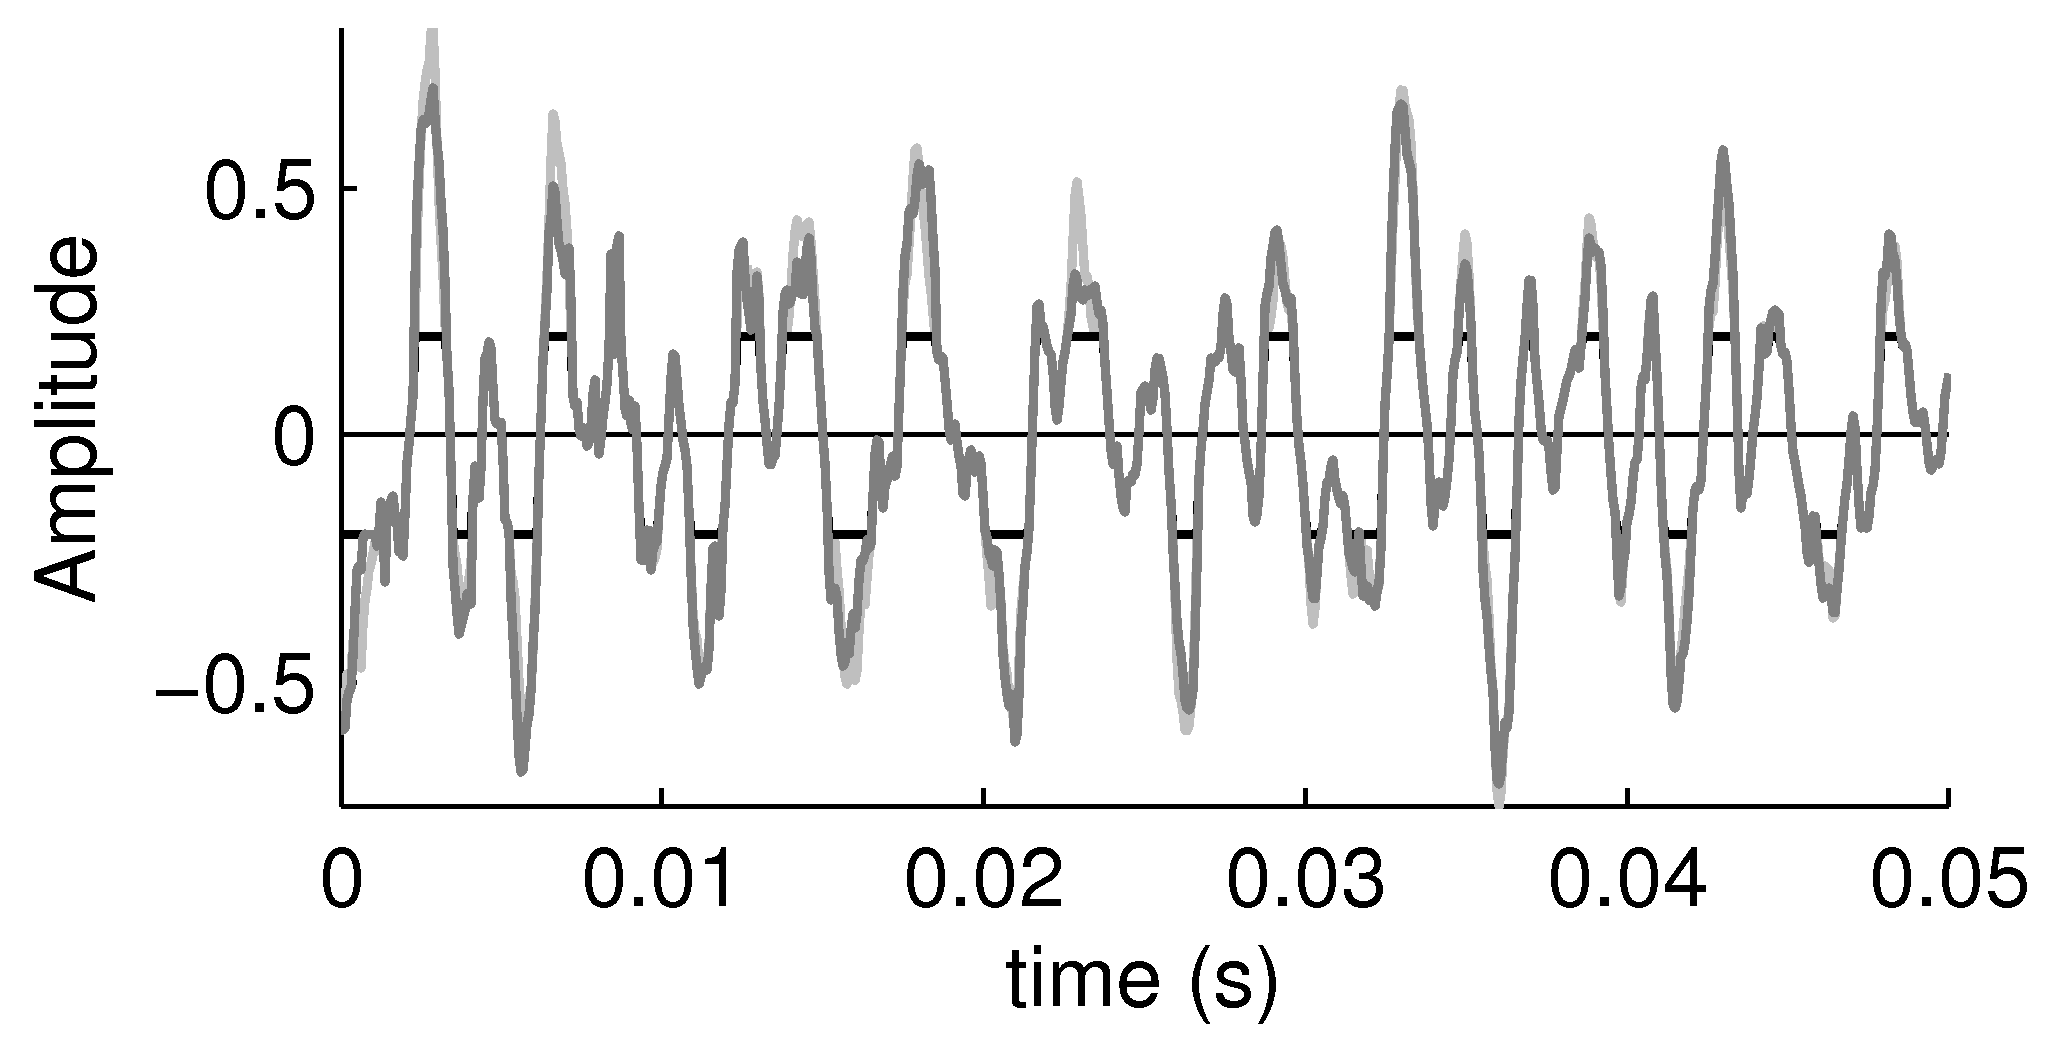
\includegraphics[width=0.9\linewidth]{audiosignal.png}
  \caption{typical audio signal}
  \label{fig:as}
\end{figure}

After the above introduction of the history of loudspeakers, let us talk about sound. Sound is a form of energy passing through air. Understanding sound is quite helpful for this project. There are two main measurements in sound, frequency and decibels. Frequency is responsible for the quality of sound in a speaker. Humans could hear audio from 20 Hz to 20 KHz, The smaller frequency is , the deeper voice is , and vice versa. The other measurement of sound which is important for a speaker is the loudness measured in dB. The higher the dB, the more our eardrum pushed inward. The interesting truth is: both a whole sound and every frequency of a sound has a dB measurement.

The last thing we will talk about is LEDs. A light-emitting diode(LED) is a semiconductor light source. When a suitable voltage is applied to the leads, electrons are able to recombine with electron holes within the device, releasing energy in the form of photons. This effect is called electroluminescence, and the color of the light (corresponding to the energy of the photon) is determined by the energy band gap of the semiconductor. the emitted lights' color will change greatly from a variety of inorganic semiconductor materials. we could produce any desired color with RGB LEDs (a tricolor LED consists of Red, Green and Blue).

This project will introduce a design that will come up with a colorful pad that could change its color and magnitude by music. The idea is quite easy whereas the point is how we could implement it. Fortunately, we made it possible at last.

\section{Related Work}

Regarding controlling LEDs by music, there has been a lot of products in the actual market. The most common one is stage lighting. It is the craft of lighting as it applies to the production of theatre, dance, opera and other performance arts. stage lighting has multiple functions including selective visibility, setting the tone of a scene and varying as music.  However, a lighting designer is required to schedule all lighting equipments including color gel, gobos, color wheels and other accessories. The light doesn't change with the music automatically in common. 

Considering the other part of the project -- speaker -- widely used in household, many kinds of home audio speakers could be found from hundreds of dollars to thousands. All the audio systems focus on performance of sound rather than visualization. It's not suitable for every scene obviously. For instance, we have a party at home as well as play music, it would be awesome if we had some light around us that could dance with music.

\section{Technical Background}

We should familiar with the technical background we used, and LED comes first. This particular type of diodes are all around us. They could convert electrical energy into light. A typical looks like Figure\ref{fig:rgbled}. The positive side of the LED is called the anode and is marked by having a longer lead or leg. The other, negative side of the LED is called the cathode. Current flows from the anode to the cathode and never the opposite direction. The brightness of an LED is directly dependent on how much current it draws. That means we could control the brightness of an LED by controlling the amount of current across it. If we connect an LED directly to a current source it will try to dissipate as much power as it?s allowed to draw, and will destroy itself. For this reason, we employ resistors that limit the flow of electrons in the circuit and protect the LED from trying to draw too much current.
\begin{figure}[ht]
  \centering
  % Requires \usepackage{graphicx}
  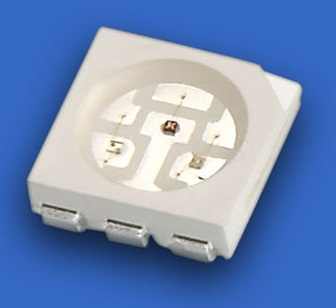
\includegraphics[width=0.9\linewidth]{rgbled.jpg}
  \caption{an Integrated RGB LED}
  \label{fig:rgbled}
\end{figure}
RGB LED is a little different, and a little tricky actually. It consists of there LEDs (Red, Green, Blue). We could change the brightness of any of them simultaneously to produce any color we desire.

The RGB color model is an color model in which red, green, and blue light are added together in various ways to reproduce a broad array of colors. The name of the model comes from the initials of the three additive primary colors, red, green, and blue. And a certain color in the RGB color model is described by indicating how much of each of the red, green, and blue is included, each component of which can vary from zero to a defined maximum value. If all the components at zero the result is black (sometimes it's' not true); if all are maximum or at the same value, the result is white. 

\section{Design Description}

The functionality of the system will be divided in four major units: The board that analyzes audio signals, the embedded microcontroller that administrates everything including the audio signal processing, controlling led display and so on, a loudspeaker to verify the functionality that our colorful pad could work well with a loudspeaker simultaneously and a LED matrix.

How to analyze audio signals is one of the most important parts in our project. Frequencies and decibels are two fundamental measurements to analyze a audio signals, therefore it's easy to pick up an idea that extract dominating information in terms of frequencies and decibels. As we know, any actual time-domain signal could be expressed into frequency-domain using the Fourier transform in terms of the amplitude of each of the frequencies that make it up. We could use this principle to estimate the bandwidth we concern about.
\begin{figure}[ht]
  \centering
  % Requires \usepackage{graphicx}
  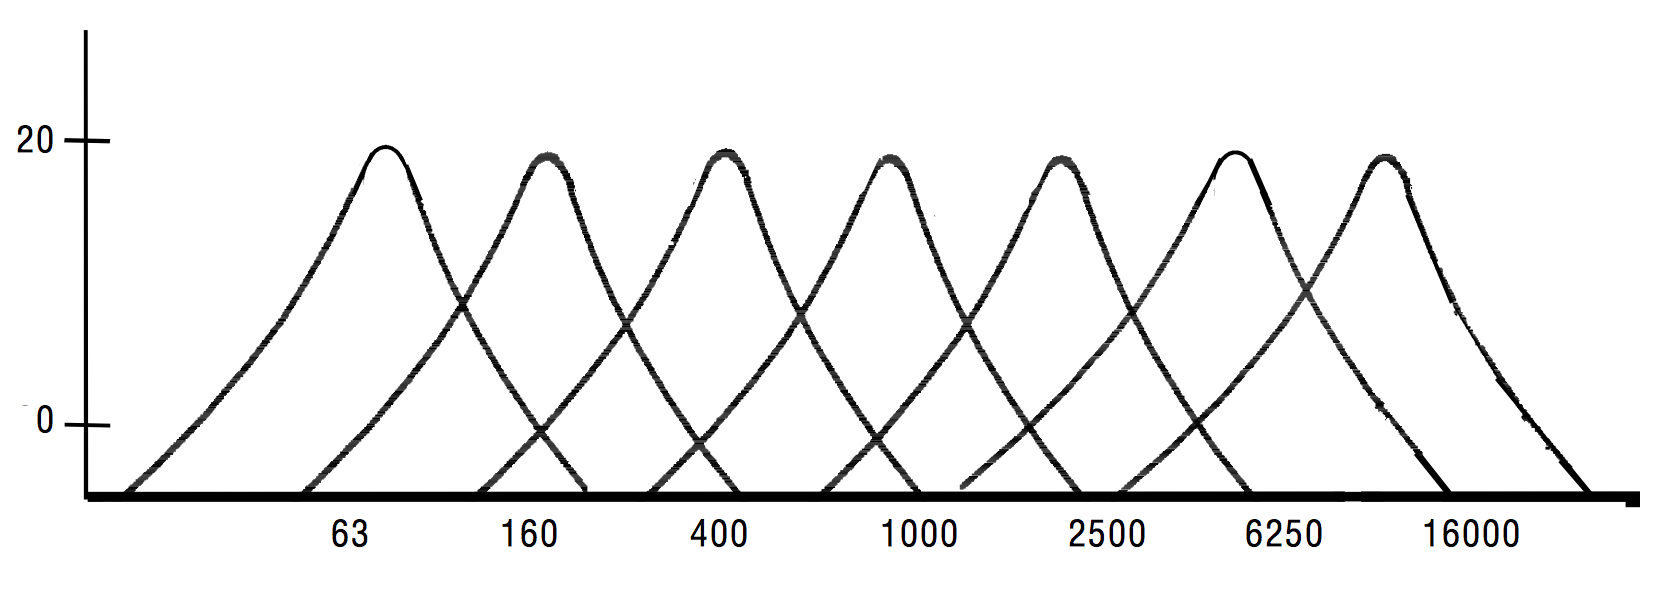
\includegraphics[width=0.9\linewidth]{frequencyaudio.png}
  \caption{seven bands of audio signal}
  \label{fig:fras}
\end{figure}

There has been plenty of chips that could implement the functions of frequency analyzing, for instance, MSGEQ7 manufactured by MSI. This chip divides the audio spectrum into seven bands, 63Hz, 160Hz, 400Hz, 1kHz, 2.5kHz, 6.25kHz and 16kHz. The seven frequencies are peak detected and multiplexed to the output to provide a DC representation of the amplitude of each band. As a typical application, it would fetch analog audio signals and output DC peak signal for measurement selected using the reset and strobe pins. Reset high resets the multiplexor. Reset low enables the strobe pin. After the first strobe leading edge, 63Hz output is on OUT. Each additional strobe leading edge advances the multiplexor one channel (63Hz, 160Hz, 400Hz, 1kHz, 2.5kHz, 6.25kHz, 16kHz etc.) and this will repeat indefinitely.
\begin{figure}[ht]
  \centering
  % Requires \usepackage{graphicx}
  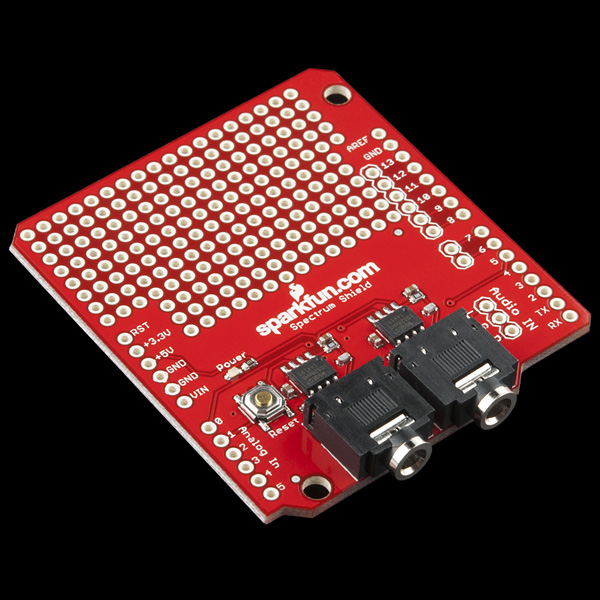
\includegraphics[width=0.7\linewidth]{spectrumshield.jpg}
  \caption{Spectrum Shield}
  \label{fig:tas4}
\end{figure}

To simply our project, we chose an intelligent control LED integrated light source called WS2812. It integrates control circuit and RGB chip together in a package forming a complete control of pixel point. Each primary color could achieve 256 brightness display to complete almost 16M color display and scan frequency not less than 400Hz/s. And it could work in cascading port transmission signal mode by single line. The technical details would be introduced in the following section.
\begin{figure}[ht]
  \centering
  % Requires \usepackage{graphicx}
  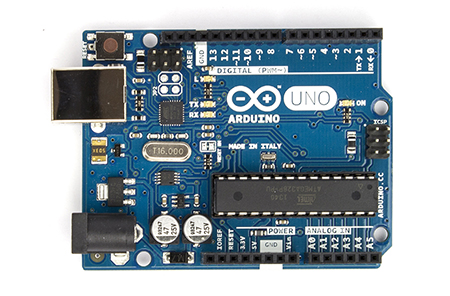
\includegraphics[width=0.9\linewidth]{arduino.jpg}
  \caption{Arduino Uno}
  \label{fig:arduino}
\end{figure}
We use the Arduino Uno as our control system. It is a microcontroller board based on the ATmega328. It has 14 digital input/output pins (of which 6 can be used as PWM outputs), 6 analog inputs, a 16 MHz ceramic resonator, a USB connection, a power jack, an ICSP header, and a reset button. It contains everything needed to support the microcontroller; simply connect it to a computer with a USB cable or power it with a AC-to-DC adapter or battery to get started.
\begin{figure}[ht]
  \centering
  % Requires \usepackage{graphicx}
  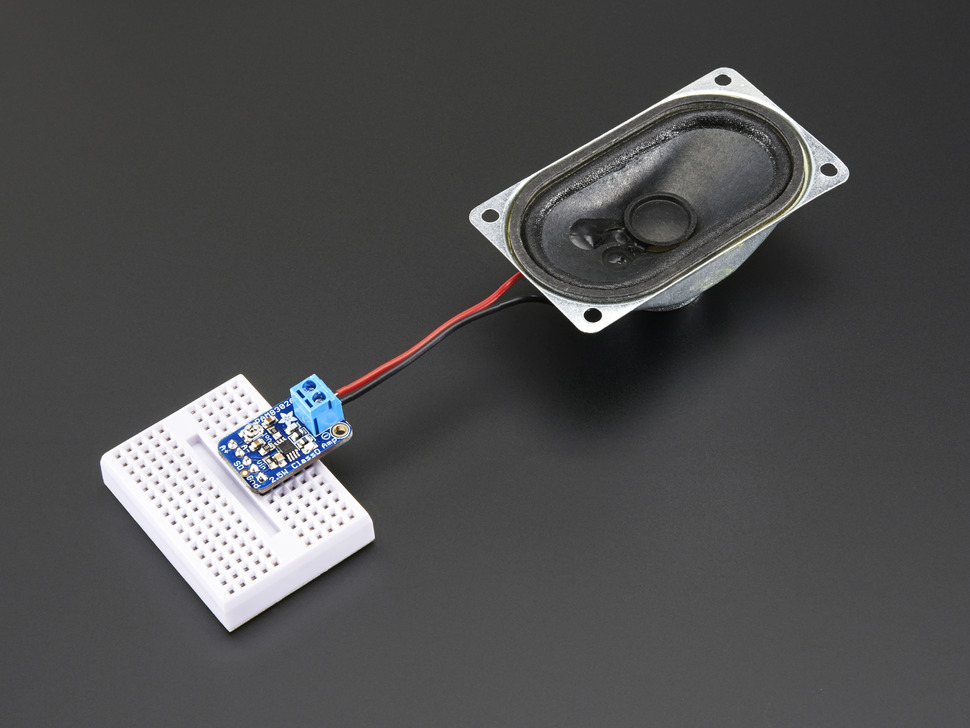
\includegraphics[width=0.9\linewidth]{audioamp.jpg}
  \caption{Audio Amplifier}
  \label{fig:aa}
\end{figure}

The last component of our project is loudspeaker sub-system consisted of a loudspeaker and an audio amplifier. we chose a 2.5W Class D Audio Amplifier to drive our loudspeaker. This amplifier is able to deliver up to 2.5 Watts speakers. The A+ and A- inputs of the amplifier go through 1.0uF capacitors, we could tie the Audio+ pin to audio signal and tie the Audio- pin to ground.

Considering the entire design procedure, requirements are required at first.

\emph{Requirement}: A basic set of requirements for the system should be satisfied: 
\begin{itemize}
\item RGB LED pixels should be arranged as a matrix and connected to each other by a single line.
\item Audio signals should be divided into seven bands using MSGEQ7.
\item Arduino Uno is used to control how the LEDs display, how the spectrum would be processed and so on.
\item LED pad may work with any typical loudspeaker together.
\end{itemize}

The basic set of requirements demonstrates the fundamental functions of the system. Briefly, both hardware and software work together to implement all the requirements.
\section{Experimental Procedures}

This section introduces that how the project is built. It should combine with two parts both hardware and software. The following steps are implemented one by one.

\emph{components testing}: To make sure all the components work well, we  verified each components we would use in our project.

\emph{The loudspeaker testing}: The speaker and audio amplifier we choosed should be tested together. We connected the speaker's +/- pins with amplifier's output pins directly. Then connected any audio source such as phone or laptop with amplifier's input pins. The power supply is almost 5 VDC to drive the amplifier.

In this part of testing, the speaker and amplifier worked well to play music from any audio source.
\begin{figure}[ht]
  \centering
  % Requires \usepackage{graphicx}
  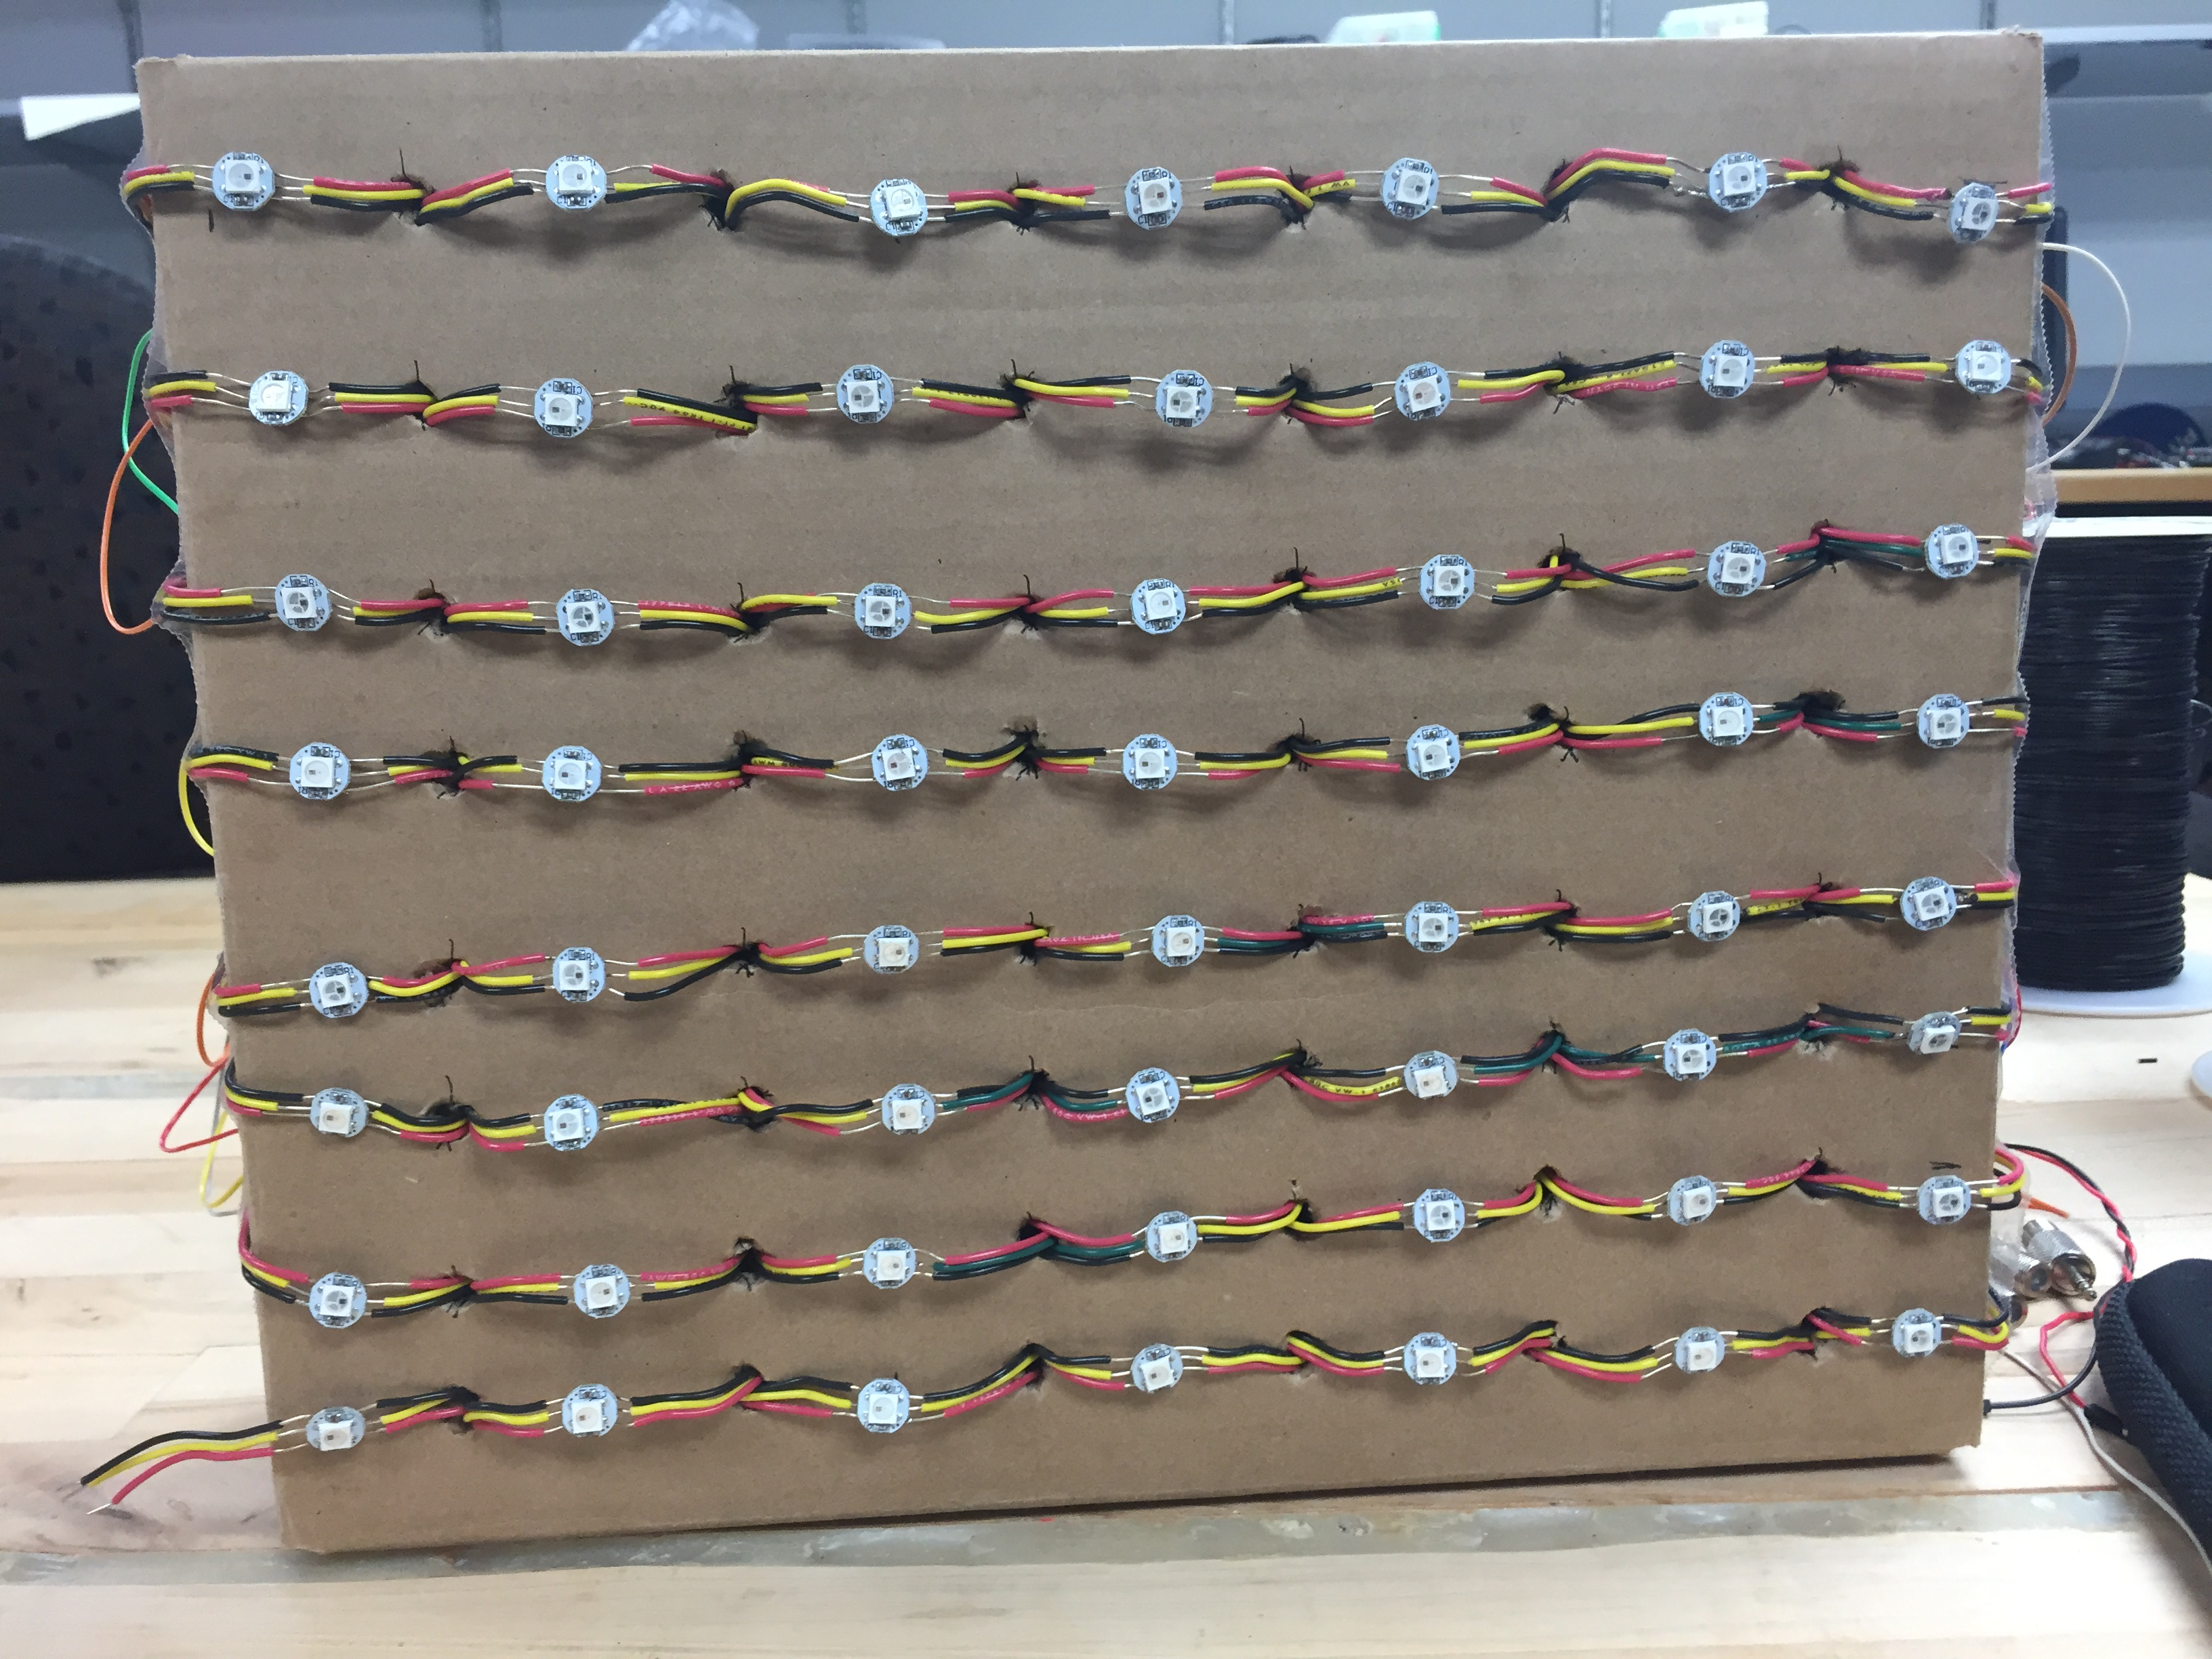
\includegraphics[width=0.7\linewidth]{ledmatrix.jpg}
  \caption{LED matrix made by ourselves}
  \label{fig:ledmat}
\end{figure}

\emph{The LED testing}: The integrated LED WS2812 is a little different from others. It would be controlled in terms of timing diagram instead of analog signal directly. Therefore, we should use Arduino Uno produce some test signal to control WS2812. We connected five chips together to verify its cascaded mode by single line. The Din pin was connected to Arduino's digital output pin. The power supply is 5VDC to drive all the color lights.

\emph{The spectrum analyzer testing}: MSGEQ7 chip is intelligent enough to obtain frequency information of audio signal. All we concern is the timing diagram and it will be discussed in the following section. to test this chip's function, Arduino Uno is also required to watch the analyzing output of spectrum shield we used. As introduce in chip's data sheet, reset and strobe pins are connected with Arduino's digital output pins and DC output is connected with Arduino's analog input pin.

The output would be display in monitor window of Arduino IDE repeatedly. we find out the output changes with the audio's melody. It proved that this chip worked as required.

At last, we should combine them together to make sure all sub-system work perfectly at the same. The number of led increased dramatically from five to seventy and they were arranged as a matrix.
\begin{figure}
  \centering
  % Requires \usepackage{graphicx}
  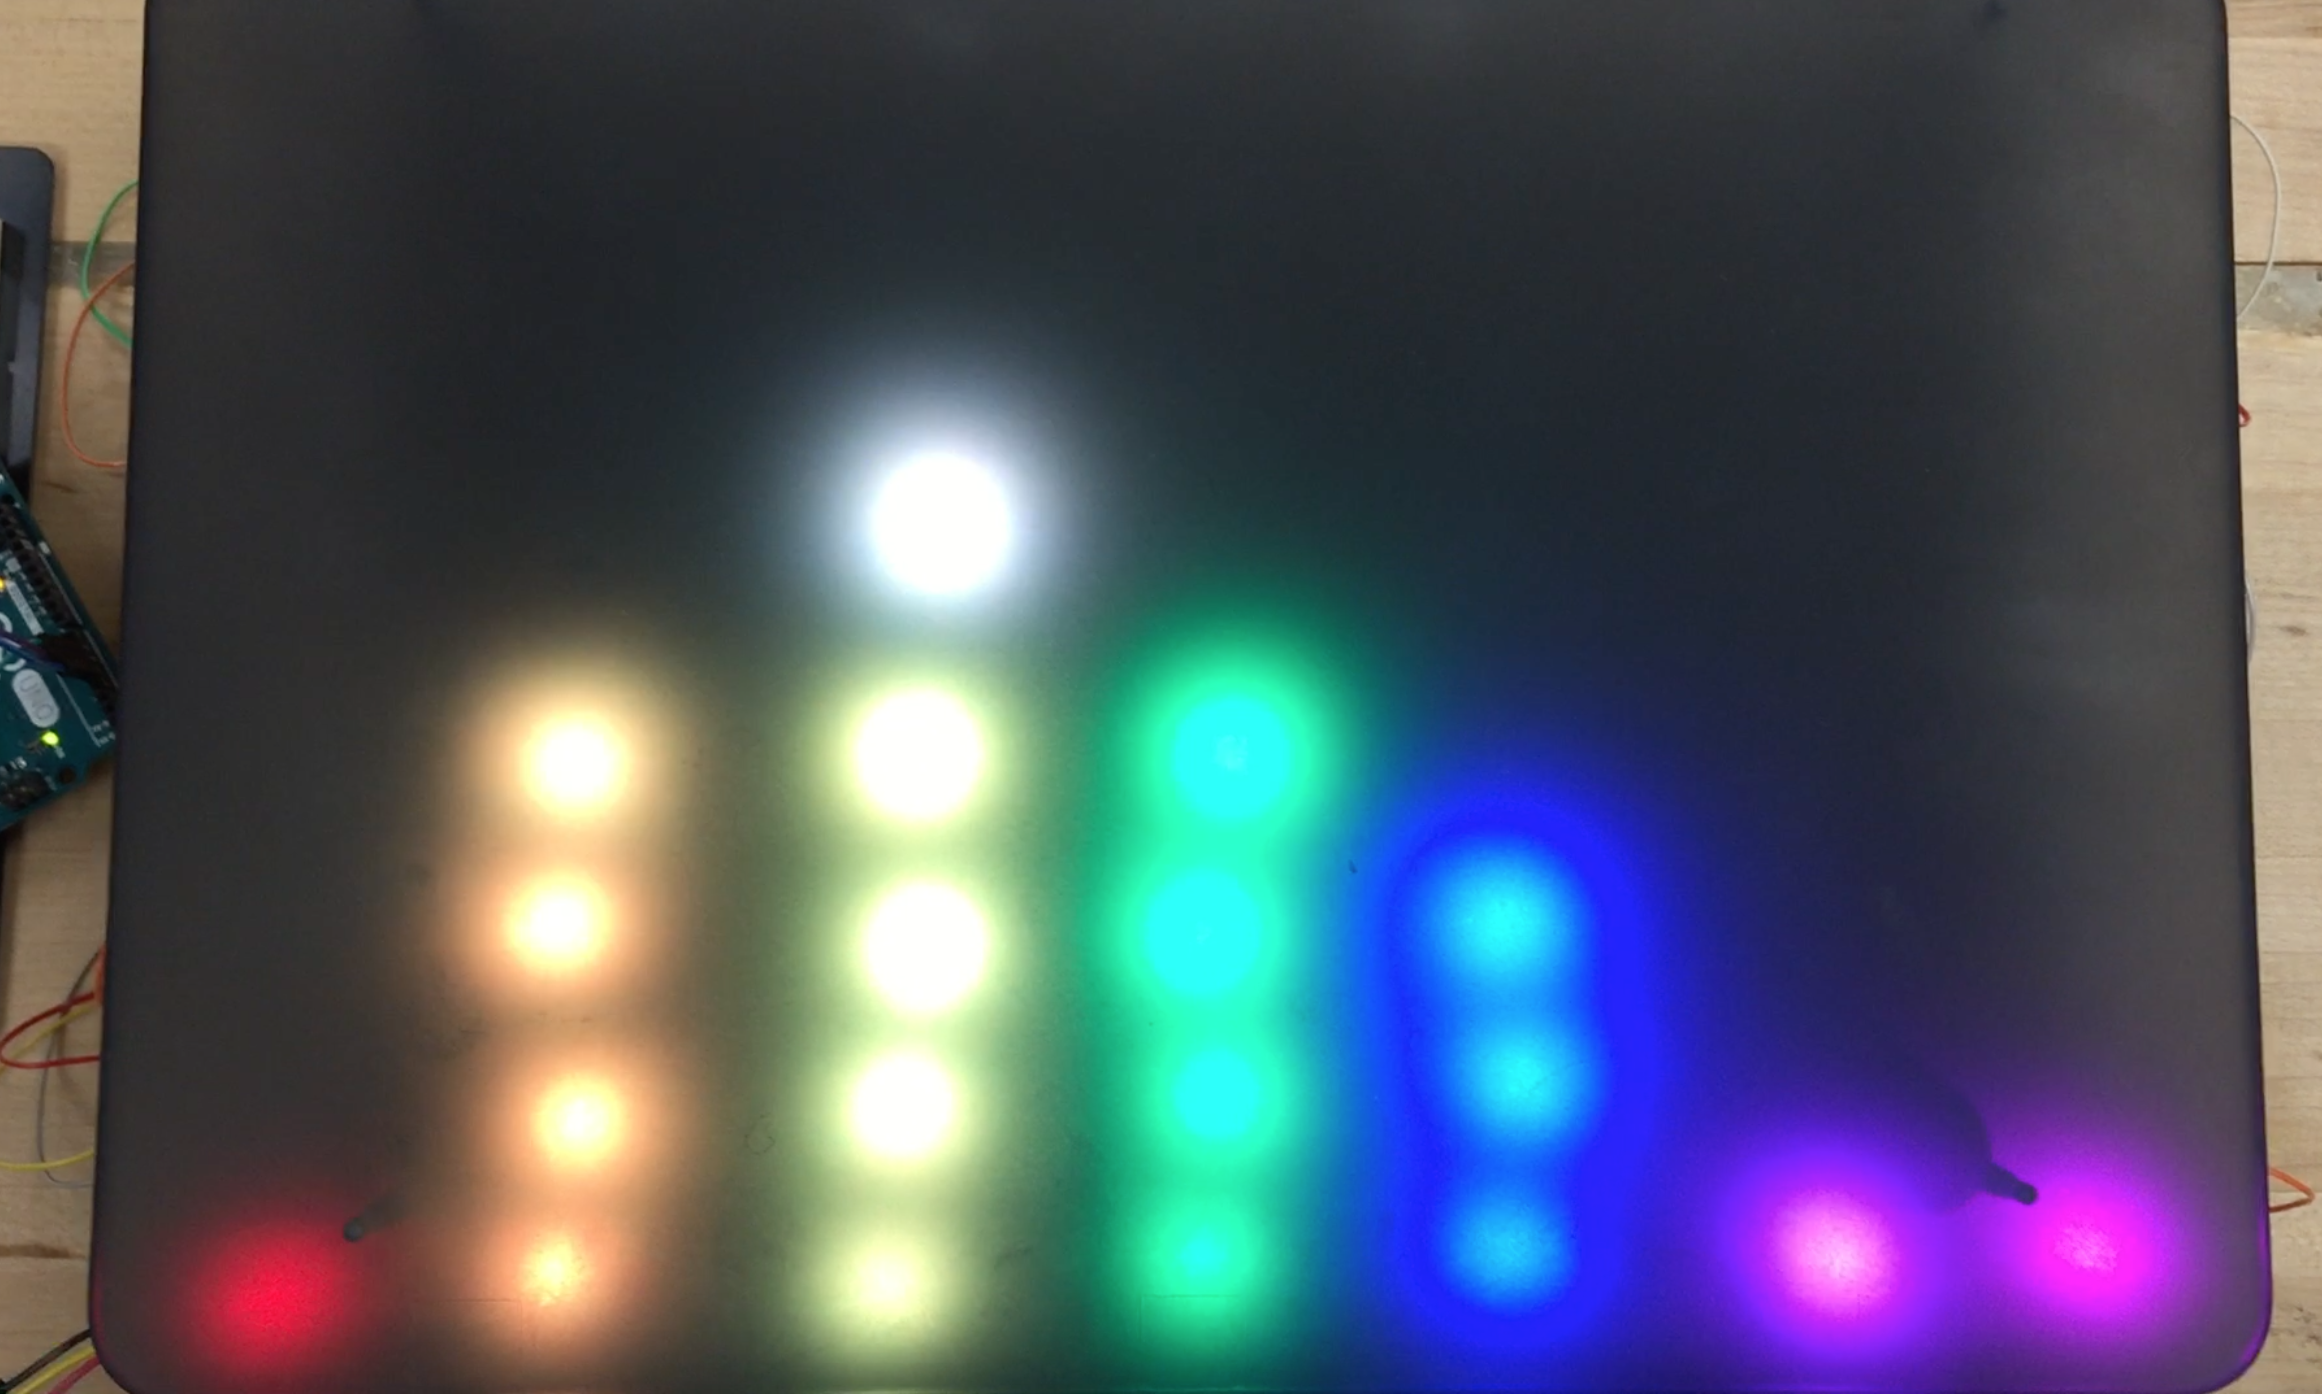
\includegraphics[width=0.7\linewidth]{result.png}
  \caption{Video Snapshot}
\end{figure}

Since our experimental results should be shown visually. A video is the best way to exhibit. We have recorded a video and  capture some images to figure out how it works. The audio signal transmitted from laptop to spectrum analyzer and was divided to different bands. The Arduino would process the result and control the LED matrix as designed. 

\section{Technology Details/Contribution}
This section will describe each of the design stages that have been implemented to stratify the system requirements. 
For the system to function as desired it has to satisfy the following points:
\begin{itemize}
\item The system has to map the frequency to 0-255 such that color can be properly displayed.
\item The system has to amplify the digital input to control the amplitude of each frequency regardless of the actual volume.
\item The system has to allow the user to upload different sounds and even vocal input.
\end{itemize}
\subsection{Hardware}
Timing requirement is the primary concern of the hardware implementation. According to the WS2812 handbook, the data transfer time of LED is $1.25\mu s \pm 600ns$. While the Arduino clock frequency is $60ns$, it's sufficient to fulfill the timing requirement of LED.

As for the spectrum shield, the MSGEQ7 strobe timing diagram shows that the strobe is enabled by the reset low and then each additional strobe leading edge advances the multiplexor one channel with seven bands. Considering the output settling time $36\mu s$, there is a delay of 1ms per band for the strobe read process.

Another issue is the LED configuration, below is a LED characteristic parameter table. The circuit utilizes a cascade method to transfer data. For a single LED, each 0-255 number is transformed into 8bits and then composite a 24bits data. Data is sent following the order of GRB in which the high bit is sent at first. For a strip, the LED number is configured and data sent by the micro-controller travel through each LED unit during a data refresh cycle.\subsection{Software}
Before communicating to the Arduino IDE, the audio signal has to be split into seven frequencies via spectrum shield. The output of the spectrum shield is an array of amplitude of each frequency. The amplitude of each frequency ranges from 0 to 1023. To utilize the amplitude to control the on/off of a LED on a strip, the amplitude has to be mapped to 0 to 255 indicating the RGB color range. Once the audio signal has been transform into digital signal and received by the Arduino IDE, a parameter scalar is applied to manipulate the amplitude such that the color pad can operate as expected even when the audio volume is too high or too low for our system. Since the LED cannot actually display black pixel {0,0,0}, the gradient color map is implemented via a HSV to RGB converter. The value(V) is fixed to 100\% to ensure that the black pixel is excluded. Each column shares the same hue(H) and elements in a column are assigned to a descending saturation(S) to form a gradient map.
\begin{figure*}
  \centering
  % Requires \usepackage{graphicx}
  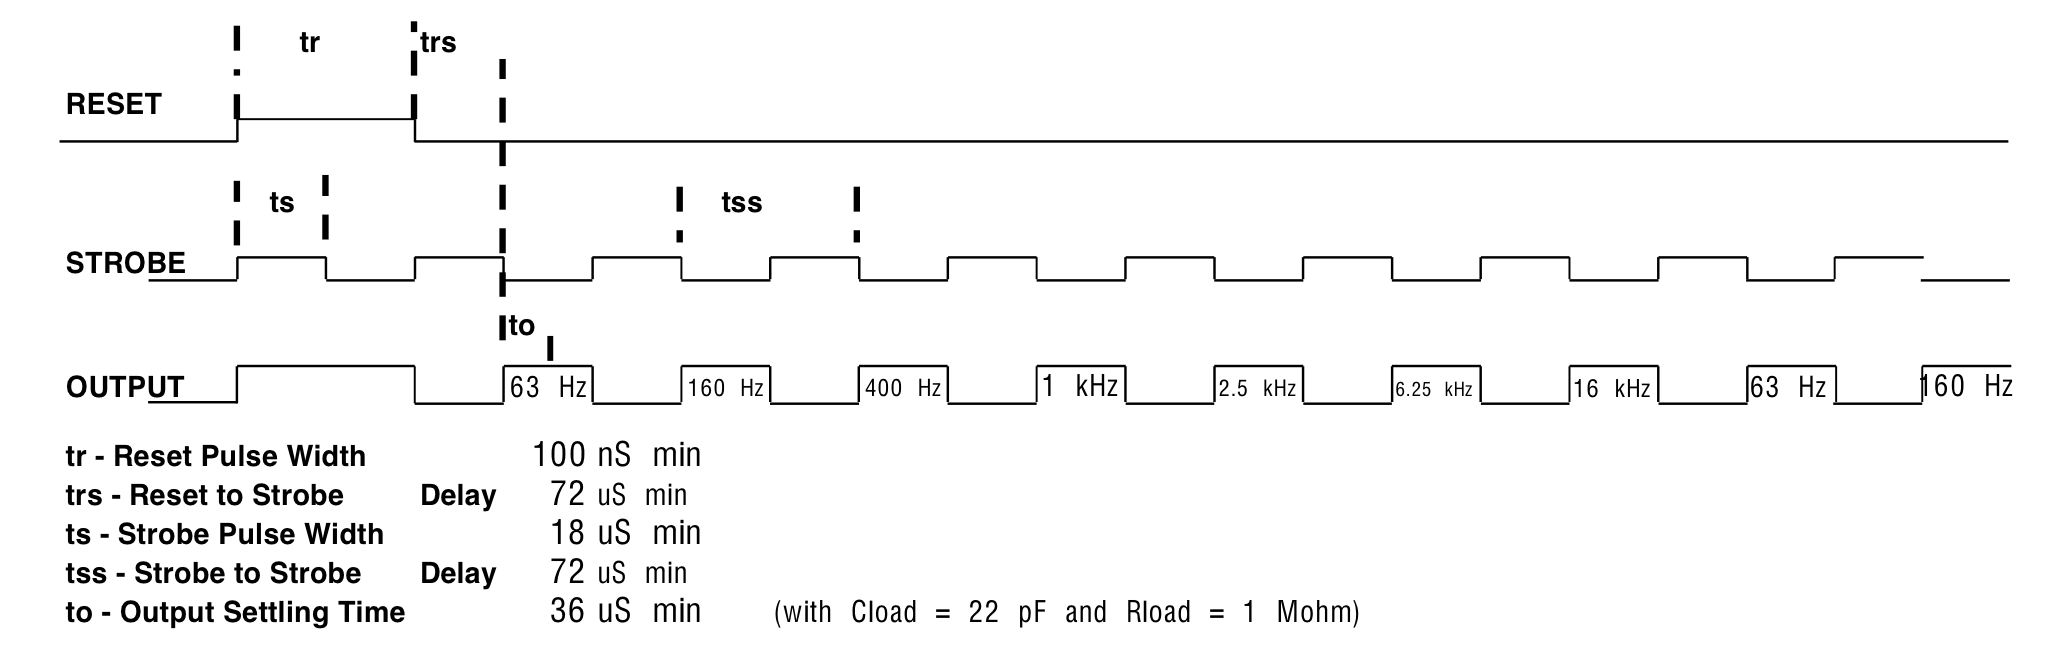
\includegraphics[width=0.7\linewidth]{timing1.png}
  \caption{Timing Diagram of Spectrum Shield}
  \label{fig:sstd1}
\end{figure*}
Another issue is the LED configuration, below is a LED characteristic parameter table.
\begin{figure*}
  \centering
  % Requires \usepackage{graphicx}
  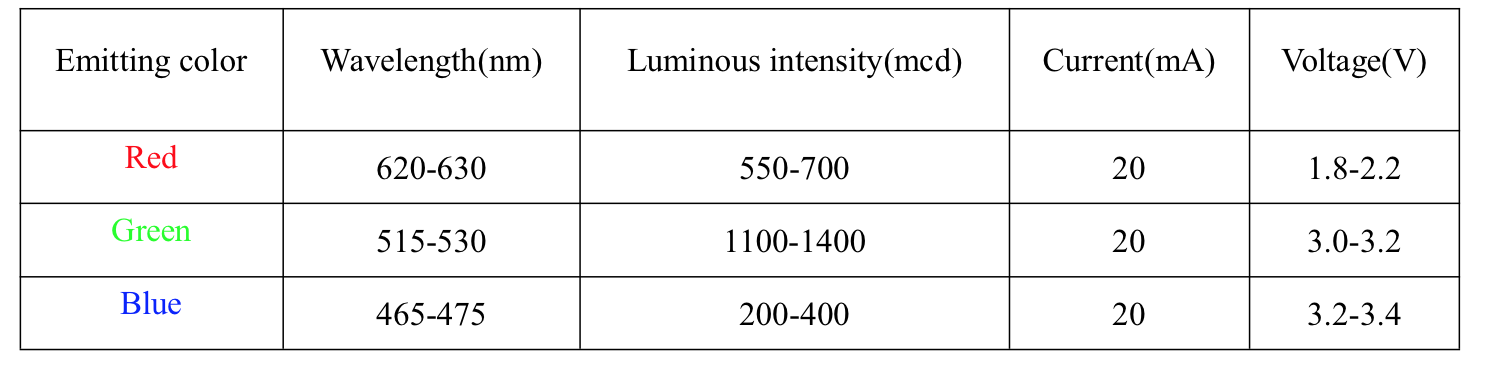
\includegraphics[width=0.7\linewidth]{ledparameter.png}
  \caption{LED characteristic parameter}
  \label{fig:ledcp}
\end{figure*}
The circuit utilizes a cascade method to transfer data. For a single LED, each 0-255 number is transformed into 8bits and then composite a 24bits data. Data is sent following the order of GRB in which the high bit is sent at first. For a strip, the LED number is configured and data sent by the micro-controller travel through each LED unit during a data refresh cycle.
\begin{figure*}
  \centering
  % Requires \usepackage{graphicx}
  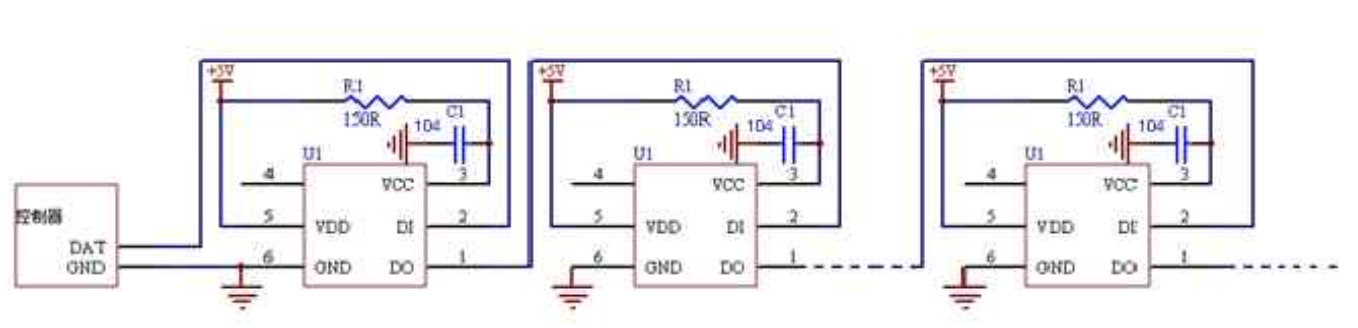
\includegraphics[width=0.7\linewidth]{ledcircuit.png}
  \caption{LED typical application circuit}
  \label{fig:ledtac}
\end{figure*}
\subsection{Software}
Before communicating to the Arduino IDE, the audio signal has to be split into seven frequencies via spectrum shield. The output of the spectrum shield is an array of amplitude of each frequency. The amplitude of each frequency ranges from 0 to 1023. To utilize the amplitude to control the on/off of a LED on a strip, the amplitude has to be mapped to 0 to 255 indicating the RGB color range.

Once the audio signal has been transform into digital signal and received by the Arduino IDE, a parameter scalar is applied to manipulate the amplitude such that the color pad can operate as expected even when the audio volume is too high or too low for our system.

Since the LED cannot actually display black pixel {0,0,0}, the gradient color map is implemented via a HSV to RGB converter. The value(V) is fixed to 100\% to ensure that the black pixel is excluded. Each column shares the same hue(H) and elements in a column are assigned to a descending saturation(S) to form a gradient map.
\subsection{Contribution}
\begin{itemize}
\item System design - Qiming
\item Hardware Purchase - Qiming
\item Hardware construction - Shuyao/Chuhan
\item Hardware implementation and debug - Shuyao/Chuhan/Qiming
\item Arduino Code design, implementation and debug - Qiming/Chuhan
\item Project Proposal - Qiming
\item Presentation - Shuyao/Chuhan/Qiming
\item Final report - Qiming/Chuhan
\item Demo Video - Shuyao/Qiming
\end{itemize}
\section{Insights}
The primary motivation of the design is to combine audioception with ophthalmoception to achieve a entertainment effect. With delicate fabrication, the fancy design can be applied to a variety of apparel and decoration, at the same it provides the possibility for people to explore their own style.

The project is dealing with analog input, the objective is to turn it into a digital signal to control the on/off of each LED. To accomplish that, the seven frequencies are peak detected and multiplexed to provide a DC representation of the amplitude of each band. During the process, a standard analog signal is transformed into frequency domain. The intermediate function is a continuous power density spectrum. To develop spectral leakage at peak frequencies, a window function is convoluted with frequency. In this case, the window function is a Gaussian function. In this way, the amplitude of seven frequencies are filtered and selected.
\section{Conclusions and Future work}
This paper presented a design for a audio controlled chromatic LED pad system. A spectrum shield is used to split the frequency that is being read by an Arduino micro-controller board and relying the results to Arduino IDE that produces the expected color index for each strobe on the pre-configured gradient color pad.
Further optimization of the hardware design may include: 
\begin{itemize}
\item Expand to dual channel to form a complete music-color map. 
\item Reverse the mater-slave relationship between audio and visual effect, e.g. using animation to produce music.
\item Utilize sensors instead of the audio input for a variety of applications e.g. using pressure sensors to play a "colorful" music just like playing a piano
\end{itemize}

% Can use something like this to put references on a page
% by themselves when using endfloat and the captionsoff option.
\ifCLASSOPTIONcaptionsoff
  \newpage
\fi

\begin{thebibliography}{1}

\bibitem {a}
MSGEQ7 Datasheet
\bibitem {b}
WS2812 Datasheet
\bibitem {c}
Arduino Website
\bibitem{d}
NeoPixel Library

\end{thebibliography}

\appendices
\section{Codes}

\begin{lstlisting}[language={C}, caption=main.cpp, keywordstyle=\color{blue!70}, commentstyle=\color{red!50!green!50!blue!50}, rulesepcolor=\color{red!20!green!20!blue!20}]
#include  "Adafruit_NeoPixel.h"

// Which pin on the Arduino is connected to the NeoPixels?
#define PIN            6
// The amplitude of how much led is work.
#define DEBUG_AMP      1.5

// MSGEQ7 Control
int strobe = 4; // strobe pins on digital 4
int res = 5; // reset pins on digital 5
int left[7]; // store band values in these arrays
int right[7];

// Use Finite State Machine to control the system
#define INIT  1
#define FREQ_1 2
#define FREQ_2 3
#define FREQ_3 4
#define FREQ_4 5

int state = FREQ_4;


// The led strip parameter
// DIM means how many leds are used to demonstrate a single frequency.
const int DIM = 8;
// FRE means the audio signal is divided to how many freqencies.
const int FRE = 7; 

// How many NeoPixels are attached to the Arduino?
#define NUMPIXELS      DIM*FRE

int led_strip_number [FRE][DIM] = {{0,13,14,27,28,41,42,55},{1,12,15,26,29,40,43,54},{2,11,16,25,30,39,44,53},{3,10,17,24,31,38,45,52},{4,9,18,23,32,37,46,51},{5,8,19,22,33,36,47,50},{6,7,20,21,34,35,48,49}};

// example for more information on possible values.
Adafruit_NeoPixel pixels = Adafruit_NeoPixel(NUMPIXELS, PIN, NEO_GRB + NEO_KHZ800);

uint32_t color[FRE][DIM];
//RED




int delayval = 500; // delay for half a second

int band;

void setup() {
  //RED
  color[0][0] = pixels.Color(255,0,0);
  color[0][1] = pixels.Color(255,26,26);
  color[0][2] = pixels.Color(255,51,51);
  color[0][3] = pixels.Color(255,77,77);
  color[0][4] = pixels.Color(255,102,102);
  color[0][5] = pixels.Color(255,128,128);
  color[0][6] = pixels.Color(255,154,154);
  color[0][7] = pixels.Color(255,179,179);
  //ORANGE
  color[1][0] = pixels.Color(255,128,0);
  color[1][1] = pixels.Color(255,141,26);
  color[1][2] = pixels.Color(255,154,51);
  color[1][3] = pixels.Color(255,166,77);
  color[1][4] = pixels.Color(255,179,102);
  color[1][5] = pixels.Color(255,192,128);
  color[1][6] = pixels.Color(255,205,154);
  color[1][7] = pixels.Color(255,218,179);
  //YELLOW
  color[2][0] = pixels.Color(255,213,0);
  color[2][1] = pixels.Color(255,218,26);
  color[2][2] = pixels.Color(255,222,51);
  color[2][3] = pixels.Color(255,226,77);
  color[2][4] = pixels.Color(255,230,102);
  color[2][5] = pixels.Color(255,235,128);
  color[2][6] = pixels.Color(255,239,154);
  color[2][7] = pixels.Color(255,243,179);
  //GREEN
  color[3][0] = pixels.Color(0,255,0);
  color[3][1] = pixels.Color(26,255,26);
  color[3][2] = pixels.Color(51,255,51);
  color[3][3] = pixels.Color(77,255,77);
  color[3][4] = pixels.Color(102,255,102);
  color[3][5] = pixels.Color(128,255,128);
  color[3][6] = pixels.Color(154,255,154);
  color[3][7] = pixels.Color(179,255,179);
  //BLUE
  color[4][0] = pixels.Color(0,0,255);
  color[4][1] = pixels.Color(26,26,255);
  color[4][2] = pixels.Color(51,51,255);
  color[4][3] = pixels.Color(77,77,255);
  color[4][4] = pixels.Color(102,102,255);
  color[4][5] = pixels.Color(128,128,255);
  color[4][6] = pixels.Color(154,154,255);
  color[4][7] = pixels.Color(179,179,255);
  //PURPLE
  color[5][0] = pixels.Color(102,0,102);
  color[5][1] = pixels.Color(153,0,153);
  color[5][2] = pixels.Color(204,0,204);
  color[5][3] = pixels.Color(255,0,255);
  color[5][4] = pixels.Color(255,51,255);
  color[5][5] = pixels.Color(255,102,255);
  color[5][6] = pixels.Color(255,153,255);
  color[5][7] = pixels.Color(255,204,204);
  //VIOLET
  color[6][0] = pixels.Color(137,0,255);
  color[6][1] = pixels.Color(148,26,255);
  color[6][2] = pixels.Color(160,51,255);
  color[6][3] = pixels.Color(172,77,255);
  color[6][4] = pixels.Color(184,102,255);
  color[6][5] = pixels.Color(196,128,255);
  color[6][6] = pixels.Color(208,154,255);
  color[6][7] = pixels.Color(220,179,255);
  
  pixels.begin(); // This initializes the NeoPixel library.
  Serial.begin(9600);
  pinMode(res, OUTPUT); // reset
  pinMode(strobe, OUTPUT); // strobe
  digitalWrite(res,LOW); // reset low
  digitalWrite(strobe,HIGH); //pin 5 is RESET on the shield
}

void readMSGEQ7() {
// Function to read 7 band equalizers
  digitalWrite(res, HIGH);
  digitalWrite(res, LOW);

  for(band=0; band <7; band++) {
    digitalWrite(strobe,LOW); // strobe pin on the shield - kicks the IC up to the next band
    delayMicroseconds(1); //
    left[band] = DEBUG_AMP*map(analogRead(0), 0, 1023, 0, 255); // store left band reading
    right[band] = DEBUG_AMP*map(analogRead(1), 0, 1023, 0, 255); // ... and the right
    digitalWrite(strobe,HIGH);
  }
}

void loop() {
  
  readMSGEQ7();
  // display values of left channel on serial monitor
  for (band = 0; band   < 7; band++) {
    Serial.print(left[band]);
    Serial.print(",");
  }
  // display values of right channel on serial monitor
  for (band = 0; band < 7; band++) {
    Serial.print(right[band]);
    Serial.print(",");
  }
  Serial.println();
  
    // For a set of NeoPixels the first NeoPixel is 0, second is 1, all the way up to the count of pixels minus one.

  switch(state){
    case INIT:
    {
      for( int i = 0; i < FRE; i++ )
      {
        for( int j = 0; j < DIM; j++ )
        {
          pixels.setPixelColor(led_strip_number[i][j], color[i][j]);
          pixels.show();
          delay(100);
        }
      }
      break;
    }
    case FREQ_1:
    {
      for(int i=0;i<NUMPIXELS;i++){
        // pixels.Color takes RGB values, from 0,0,0 up to 255,255,255
        int test=left[5]/42;
        int amp = test>i?20:0;
        int pick = random(1,4);
        switch(pick){
          case 1: pixels.setPixelColor(i, pixels.Color(0,amp,0)); break;
          case 2: pixels.setPixelColor(i, pixels.Color(amp,0,0)); break;
          default: pixels.setPixelColor(i, pixels.Color(0,0,amp)); 
        }  
        pixels.show(); // This sends the updated pixel color to the hardware.
      }
      break;
    }
    case FREQ_2:
    {
      //The amplitude of one frequency is sliced to DIM sections
      int FRE_SLICE = 255/DIM;

      for (int i = 0; i < FRE; ++i)
      {
        int dim_max = left[i]/FRE_SLICE;
        for (int j = 0; j < DIM; ++j)
        {
          // The jth leds should be lighted or not
          int amp = dim_max > j ? 100 : 0;
          int pick = random(1,4);
          switch(pick){
            case 1: pixels.setPixelColor(led_strip_number[i][j], pixels.Color(0,amp,0)); break;
            case 2: pixels.setPixelColor(led_strip_number[i][j], pixels.Color(amp,0,0)); break;
            default: pixels.setPixelColor(led_strip_number[i][j], pixels.Color(0,0,amp)); 
        }  
        }
      }
      pixels.show();
      break;
    }
    //FREQ_3
        case FREQ_3:
    {
      //The amplitude of one frequency is sliced to DIM sections
      int FRE_SLICE = 255/DIM;

      for (int i = 0; i < FRE; ++i)
      {
        int dim_max = left[i]/FRE_SLICE;
        for (int j = 0; j < DIM; ++j)
        {
          // The jth leds should be lighted or not
          int amp = dim_max > j ? 150 : 0;
          pixels.setPixelColor(led_strip_number[i][j], pixels.Color(amp,0,0));
        }  
        }
      pixels.show();
      break;
    }
        //FREQ_4
        case FREQ_4:
    {
      //The amplitude of one frequency is sliced to DIM sections
      int FRE_SLICE = 255/DIM;

      for (int i = 0; i < FRE; ++i)
      {
        int dim_max = left[i]/FRE_SLICE;
        for (int j = 0; j < DIM; ++j)
        {
          // The jth leds should be lighted or not
          uint32_t amp = dim_max > j ? color[i][j]: 0;
          pixels.setPixelColor(led_strip_number[i][j], amp);
        }  
        }
      pixels.show();
      break;
    }
    }
}
\end{lstlisting}




\end{document}


